\begin{figure}[t]
    \centering
    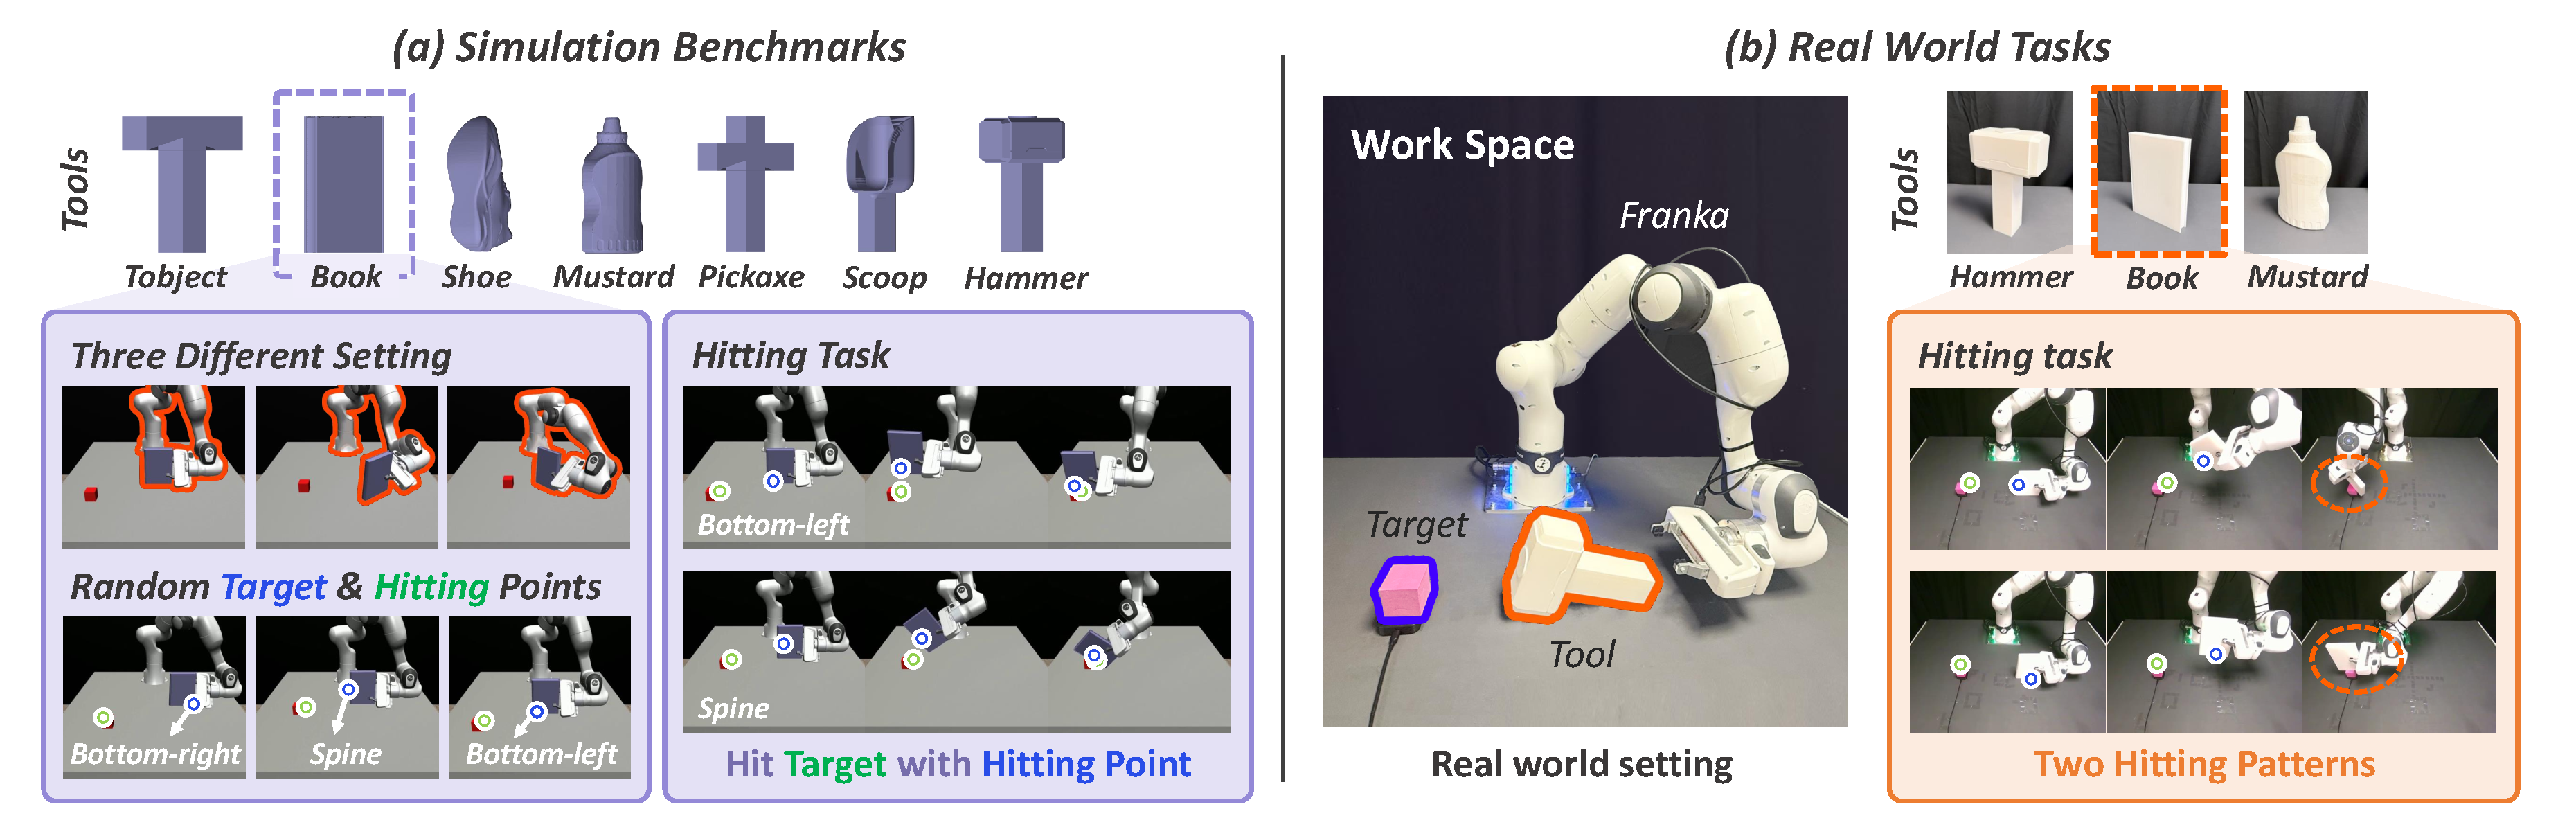
\includegraphics[width=\linewidth]{figures/experiments_settings.pdf}
    \caption{
    \textbf{Simulation Benchmark and Real-world Setting.} (a) The simulation benchmark contains seven tools, three initial settings per tool, and randomized target and hitting points. (b) The real-world setting uses a Franka robot and includes three tools, each with two hitting patterns.
    }
    \label{fig:experiment_settings}
\end{figure}
\section{Experiments}
\label{sec:experiments}

% \lw{We design our experiments to test four hypotheses that together validate the central claims of this work.
% \begin{itemize}[leftmargin=*]
%     \item \textbf{H1: End-to-end policies fail at functional generalization; an intermediate representation is necessary.} Tested by the main comparison against FM and DP (Tab.~\ref{tab:simulation_results}).
%     \item \textbf{H2: Among candidate intermediate representations, 2D keypoint trajectories best balance affordance expressiveness and action groundability.} Tested by the representation ablation (Tab.~\ref{tab:ablation_intermediate_representation}).
%     \item \textbf{H3: Keypoint trajectories must be function-aware; generic keypoint tracking is not enough.} Tested by the comparison against ATM, which uses pretrained generic keypoints (Tab.~\ref{tab:simulation_results}).
%     \item \textbf{H4: The two-stage design generalizes under moderate action-labeled tool diversity, making it a practical recipe for tool-use learning.} Tested by the tool-diversity ablation (Tab.~\ref{tab:ablation_tool_generalization_setting}).
% \end{itemize}}

Functional generalization remains a largely underexplored problem in robotic manipulation.
In this work, we instantiate it with the hitting function and construct both simulation and real-world benchmarks to systematically evaluate whether a policy can transfer the same function to unseen tools. Specifically, we design experiments to test four hypotheses that together validate the central claims of this work:
\begin{itemize}[leftmargin=*]
    \item \textbf{H1}: Functional generalization requires an intermediate representation, not end-to-end mapping.
    %Tested by the main comparison against FM and DP (Tab.~\ref{tab:simulation_results}).
    \item \textbf{H2}: Among candidate intermediate representations, 2D keypoint trajectories best balance affordance expressiveness and action groundability.
    % Tested by the representation ablation (Tab.~\ref{tab:ablation_intermediate_representation}).
    \item \textbf{H3}: Keypoint trajectories must be function-aware; generic keypoint tracking is not enough.
    % Tested by the comparison against ATM, which uses pretrained generic keypoints (Tab.~\ref{tab:simulation_results}).
    \item \textbf{H4}: The two-stage design generalizes under moderate action-labeled tool diversity, making it a practical recipe for tool-use learning.
    % Tested by the tool-diversity ablation (Tab.~\ref{tab:ablation_tool_generalization_setting}).
\end{itemize}

\subsection{Experimental setup}
% Functional generalization remains a largely underexplored problem in robotic manipulation.
% In this work, we instantiate it with the hitting function and construct both simulation and real-world benchmarks to systematically evaluate whether a policy can transfer the same function to unseen tools. \lw{move to first paragraph}



%\paragraph{Simulation Benchmark.}
\textbf{Simulation Benchmark.}~~
% As shown in Fig.~\ref{fig:experiment_settings}, our simulation benchmark contains seven tools, each with three different initial settings.
% For each setting, we collect 30 demonstrations, resulting in 630 samples in total.
% In each sample, the positions of the target cube and the tool-specific hitting point are randomly initialized.
% Our main setting trains all methods on four tools, including hammer, tobject, pickaxe, and mustard, and evaluates their functional generalization performance on the remaining three unseen tools.
% During evaluation, a rollout is considered successful only when the tool strikes the target cube using the designated hitting point.
%For each tool-setting pair, we  \lw{how do we collect data? add MPPI here} 30 demonstrations, resulting in 630 demonstrations in total.
As shown in Fig.~\ref{fig:experiment_settings}, our simulation benchmark contains 7 tools, each with 3 different initial settings. 
For each tool-setting pair, we collect 30 demonstrations using a four-stage Model Predictive Path Integral (MPPI) planner, resulting in 630 demonstrations in total. The MPPI planner generates an action trajectory by optimizing stage-dependent objectives that sequentially encourage the robot to lift the tool, move it toward the target, align the tool-specific hitting point with the target cube, and execute the final strike. In each demonstration, we randomly initialize the target cube position and sample the tool-specific hitting point along the tool boundary, requiring the policy to adapt its motion to both the tool geometry and the target location. In the main setting, all methods are trained on 4 tools, including hammer, tobject, pickaxe, and mustard, and evaluated on the remaining 3 unseen tools. During evaluation, each unseen tool is tested under three initial settings with 30 rollout episodes. A rollout is considered successful only if the robot strikes the target cube using the designated hitting point.



% \paragraph{Real-World Setting.}
\textbf{Real-World Setting.}~~
% Our real-world setting is constructed on a Franka robot platform and includes three tools: hammer, mustard, and book.
% As shown in Fig.~\ref{fig:experiment_settings}, each tool contains two hitting patterns, and each pattern contains 20 expert demonstrations, resulting in 120 real-world trajectories.
% We train the policy on hammer and mustard data and evaluate its functional generalization ability on the unseen book tool.
% A trial is considered successful only if the robot uses the specified hitting pattern to strike the target cube.
% \lw{sys2 data is action free, we can use human videos to collect data}
We further construct a real-world benchmark on a Franka robot platform, as shown in Fig.~\ref{fig:experiment_settings}. 
The real-world setting contains 3 tools: hammer, mustard, and book. 
Each tool has two hitting patterns, and each pattern contains 20 expert demonstrations, resulting in 120 real-world trajectories.
We train the policy on hammer and mustard and evaluate its functional generalization ability on the unseen book tool. 
For each hitting pattern, we perform 20 real-world rollout trials. A trial is successful if the robot follows the specified hitting pattern and strikes the target.

\textbf{Baselines.}~~We compare \algoname{} against three baselines covering end-to-end and keypoint-based policies. \textit{Flow-Matching (FM)}~\cite{lipmanflow} and \textit{Diffusion Policy (DP)}~\cite{chi2025diffusion} are end-to-end visuomotor policies that map observations directly to actions, serving as references for the perception-to-action gap (Sec.~\ref{sec:intro}). \textit{ATM}~\cite{wen2023any} also conditions on keypoint trajectories, but obtains them from a generic tracker pretrained on LIBERO-90 rather than a function-aware predictor, allowing us to test whether the gain comes from using keypoints or from predicting function-aware keypoint motion. All baselines receive the same inputs as \algoname{}: visual observations, proprioceptive states, and the initial hitting and target point positions.

%\paragraph{Evaluation Metrics.}
\textbf{Evaluation Metrics.}~~
All experiments report the success rate (SR) as the main evaluation metric, which is defined as the number of successful trials divided by the total number of rollout trials.

% For a fair comparison, in both simulation and real-world experiments, all policies are given the same input conditions, including visual observations, robot proprioceptive states, and the initial positions of the hitting point and target point.


% \begin{table}[t]
% \centering
% \caption{Performance comparison on simulation and real-world tools.}
% \label{tab:exp_main_results}
% \resizebox{0.8\linewidth}{!}{
% \begin{tabular}{lccccc}
% \toprule
% \multirow{2}{*}{Method} 
% & \multicolumn{4}{c}{Simulation Tools} 
% & \multicolumn{1}{c}{Real-World Tools} \\
% \cmidrule(lr){2-5} \cmidrule(lr){6-6}
% & Scoop & Shoe & Book & Avg. & Book \\
% \midrule
% Flow-Matching    & 0.07 & 0.03 & 0.16 & 0.09 & -- \\
% Diffusion Policy & 0.18 & 0.08 & 0.27 & 0.17 & -- \\
% \hline
% ATM              & -- & -- & -- & -- & -- \\
% \hline
% \algoname{} (Ours)      & 0.42 & 0.23 & 0.42 & 0.36 & -- \\
% \bottomrule
% \end{tabular}
% }
% \end{table}


% \begin{table}[ht]
% \centering
% \caption{\textbf{Simulation Results.} We conduct experiments on three unseen tools, including Scoop, Shoe, and Book. Each unseen tool contains three different initial settings. We perform 30 rollout episodes for each setting and report the success rate.}
% \label{tab:simulation_results}
% \resizebox{0.9\linewidth}{!}{
% \begin{tabular}{lcccccccccc}
% \toprule
% \multirow{2}{*}{Method} 
% & \multicolumn{3}{c}{Scoop} 
% & \multicolumn{3}{c}{Shoe} 
% & \multicolumn{3}{c}{Book} 
% & \multirow{2}{*}{Avg} \\
% \cmidrule(lr){2-4} 
% \cmidrule(lr){5-7} 
% \cmidrule(lr){8-10}
% & S01 & S02 & S03 
% & S01 & S02 & S03 
% & S01 & S02 & S03 
% & \\
% \midrule
% Flow-Matching 
% & 0.00 & 0.03 & 0.17 
% & 0.00 & 0.07 & 0.03 
% & 0.13 & 0.17 & 0.17 
% & \cellcolor{gray!15}0.09 \\

% DP 
% & 0.13 & 0.13 & 0.27 
% & 0.00 & 0.13 & 0.10 
% & 0.33 & \textbf{0.23} & 0.23 
% & \cellcolor{gray!15}0.17 \\

% \midrule
% ATM 
% & 0.13 & 0.17 & 0.07 
% & 0.10 & 0.00 & 0.07 
% & 0.07 & 0.07 & 0.03 
% & \cellcolor{gray!15}0.08 \\

% \midrule
% \algoname{} (Ours) 
% & \textbf{0.30} & \textbf{0.30} & \textbf{0.67} 
% & \textbf{0.23} & \textbf{0.23} & \textbf{0.23} 
% & \textbf{0.53} & 0.20 & \textbf{0.53} 
% & \cellcolor{gray!18}\textbf{0.36} \\
% \bottomrule
% \end{tabular}
% }
% \end{table}

\begin{table}[ht]
\centering
\caption{\textbf{Simulation Results.} Success rate (SR) on three unseen tools. Each setting is evaluated with 30 rollouts, and setting-level SR, tool-level average SR, and overall average SR are reported.}
\label{tab:simulation_results}
\resizebox{\linewidth}{!}{
\begin{tabular}{lccccccccccccc}
\toprule
\multirow{2}{*}{Method} 
& \multicolumn{4}{c}{Scoop} 
& \multicolumn{4}{c}{Shoe} 
& \multicolumn{4}{c}{Book} 
& \multirow{2}{*}{Overall} \\
\cmidrule(lr){2-5} 
\cmidrule(lr){6-9} 
\cmidrule(lr){10-13}
& S01 & S02 & S03 & Avg.
& S01 & S02 & S03 & Avg.
& S01 & S02 & S03 & Avg.
& \\

\midrule
FM~\cite{lipmanflow} 
& 0.00 & 0.03 & 0.17 & \cellcolor{gray!15}0.07
& 0.00 & 0.07 & 0.03 & \cellcolor{gray!15}0.03
& 0.13 & 0.17 & 0.17 & \cellcolor{gray!15}0.16
& \cellcolor{teal!10}0.09 \\

DP~\cite{chi2025diffusion} 
& 0.13 & 0.13 & 0.27 & \cellcolor{gray!15}0.18
& 0.00 & 0.13 & 0.10 & \cellcolor{gray!15}0.08
& 0.33 & \textbf{0.23} & 0.23 & \cellcolor{gray!15}0.26
& \cellcolor{teal!10}0.17 \\

\midrule
ATM~\cite{wen2023any} 
& 0.13 & 0.17 & 0.07 & \cellcolor{gray!15}0.12
& 0.10 & 0.00 & 0.07 & \cellcolor{gray!15}0.06
& 0.07 & 0.07 & 0.03 & \cellcolor{gray!15}0.06
& \cellcolor{teal!10}0.08 \\

\midrule
\algoname{} (Ours) 
& \textbf{0.30} & \textbf{0.30} & \textbf{0.67} & \cellcolor{gray!18}\textbf{0.42}
& \textbf{0.23} & \textbf{0.23} & \textbf{0.23} & \cellcolor{gray!18}\textbf{0.23}
& \textbf{0.53} & 0.20 & \textbf{0.53} & \cellcolor{gray!18}\textbf{0.42}
& \cellcolor{teal!10}\textbf{0.36} \\
\bottomrule
\end{tabular}
}
\end{table}


\begin{figure}[ht]
    \centering
    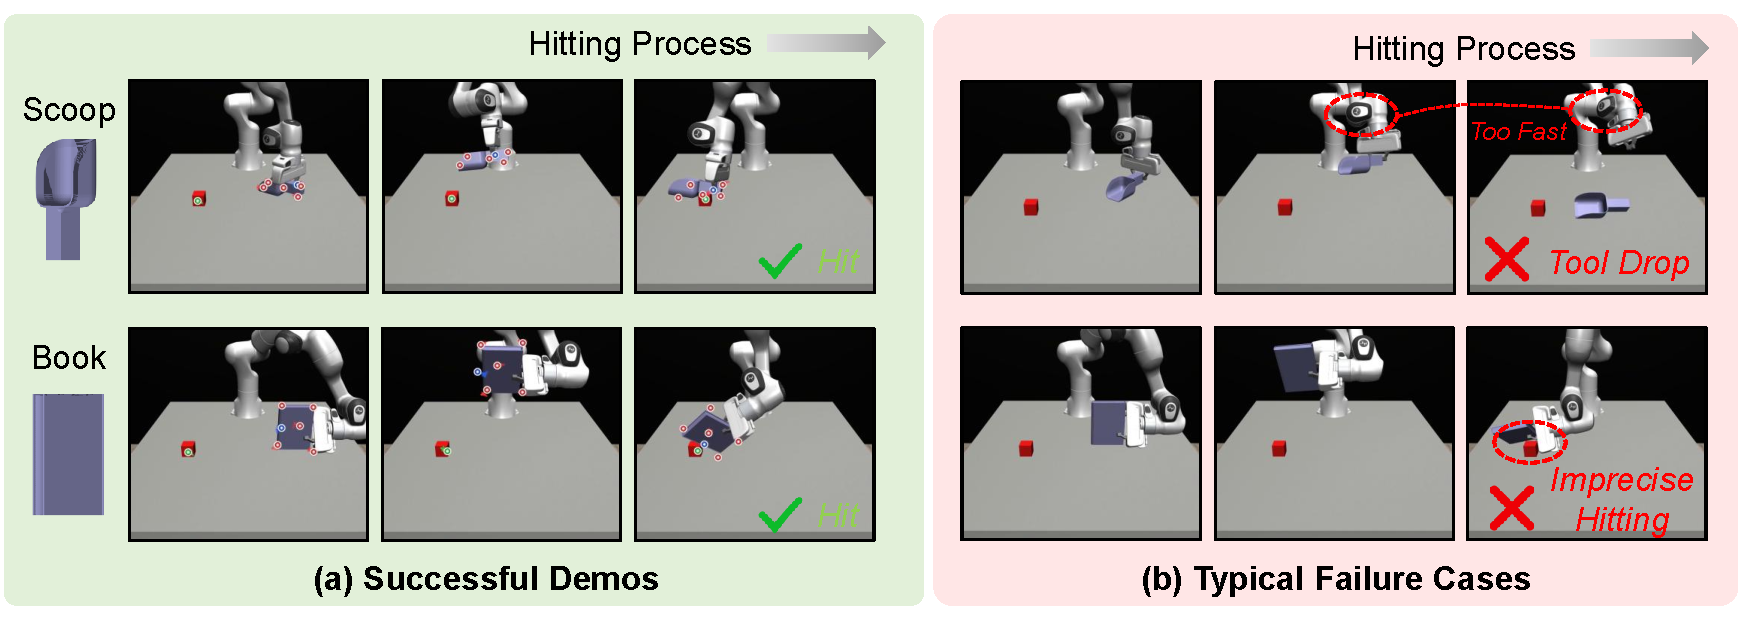
\includegraphics[width=1.0\linewidth]{figures/qualitative-results.pdf}
    \caption{\textbf{Qualitative results of \algoname{}.} (a) Successful demos with predicted keypoint-based functional plans on unseen tools. (b) Two typical failure cases of \algoname{}.}

    \label{fig:qualitative-analysis}
\end{figure}


\begin{figure}[t]
    \centering
    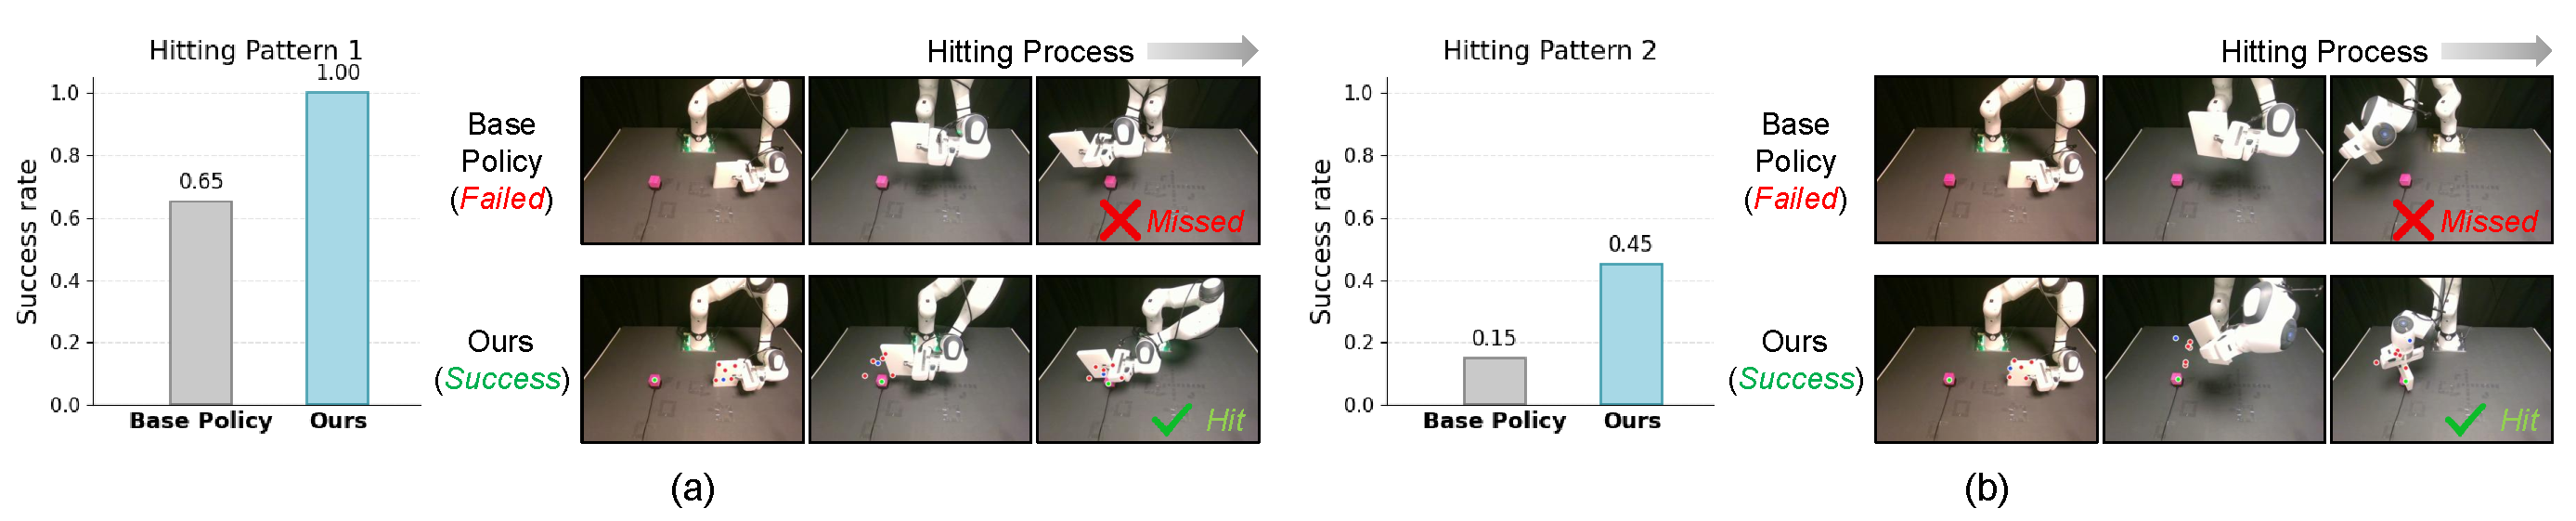
\includegraphics[width=1.0\linewidth]{figures/real-world-exp.pdf}
    \caption{\textbf{Real-World Results.} Results on the unseen book across two hitting patterns. We compare \algoname{} with the FM base policy. Results for hitting with (a) the bottom. (b) the spine.}
    \label{fig:real-world-results}
\end{figure}



% \subsection{Main Results \lw{\& Analysis}}
\subsection{Main Results \& Analysis}

% We compare \algoname{} with state-of-the-art diffusion-based and flow-matching-based policy learning methods. For a fair comparison, all methods are trained with the same input conditions, including visual observations, robot proprioceptive states, and the initial positions of the hitting point and target point. We train all methods on samples from four tools, including hammer, tobject, dtobject, and mustard, and evaluate their generalization performance on the remaining three unseen tools.


%\paragraph{Simulation Results.}
% \textbf{Simulation Results.}~~ We compare \algoname{} with Flow-Matching (FM)~\cite{lipmanflow}, Diffusion Policy (DP)~\cite{chi2025diffusion}, and the keypoint-based policy ATM~\cite{wen2023any}. For a fair comparison, all policies take the same inputs, including observations, robot proprioceptive states, and initial keypoints.
% As shown in Tab.~\ref{tab:simulation_results}, both FM and DP show limited performance on hitting-function generalization, indicating that directly mapping visual observations to actions struggles to transfer across tools.
% For ATM, we use its tracking module pretrained on LIBERO-90 and only fine-tune the track-guided policy on our benchmark.
% Since the pretrained tracking module lacks prior knowledge of the hitting function, it cannot effectively reason about function-relevant keypoint trajectories to guide the low-level policy, even with initial keypoints.
% In contrast, through action-free pretraining, \algoname{} learns the underlying intent of the hitting function and predicts structured functional plans that generalize across tools. By grounding these plans into precise actions, \algoname{} substantially improves the success rate on unseen tools, outperforming the second-best method (DP) by 19\% in overall SR.

% %\paragraph{Real-World Results.} 
% \textbf{Real-World Results.}~~We further compare \algoname{} with the Base Policy (FM) in the real world.
% As shown in Fig.~\ref{fig:real-world-results}, \algoname{} consistently outperforms FM under both hitting patterns.
% The typical failure cases show that, relying only on observations, FM struggles to align the hitting region of novel tools with the target, leading to missed hits.
% In contrast, guided by the predicted keypoint-based functional plans, \algoname{} achieves more accurate alignment and completes the hitting task.

\textbf{Simulation Results.}~~As shown in Tab.~\ref{tab:simulation_results}, FM and DP achieve only $0.09$ and $0.17$ average SR on unseen tools, validating \textbf{H1}: without an intermediate representation exposing the contact region and its alignment with the target, end-to-end policies fall back on the motor patterns of the most visually similar seen tool. 
ATM also underperforms ($0.08$), validating \textbf{H3}: its generic tracker cannot anticipate function-relevant motion, so the keypoint trajectories it provides fail to describe how the contact region should approach the target. 
In contrast, \algoname{} achieves $0.36$, outperforming DP by over $2\times$ with consistent gains across all three unseen tools, and Fig.~\ref{fig:qualitative-analysis}~(a) shows that its predicted keypoint trajectories explicitly bring the tool-specific contact region toward the target before impact. 
We further observe two failure modes (Fig.~\ref{fig:qualitative-analysis}~(b)): \textit{imprecise hitting}, where the 2D trajectories capture the overall motion but lack fine-grained spatial alignment, motivating 3D-aware functional representations; and \textit{tool dropping}, where the execution policy produces jerky actions, motivating smoothness regularization or trajectory post-processing.


% \textbf{Simulation Results.}
% As shown in Tab.~\ref{tab:simulation_results}, the end-to-end policies FM and DP achieve limited success rates on unseen tools. This validates \textbf{H1}, showing that directly mapping visual observations to actions is insufficient for functional generalization. Although the unseen tools share the same hitting function as the seen tools, their geometries, hitting regions, and required motions differ substantially. As a result, FM and DP often fail to infer how the tool-specific hitting region should be aligned with the target, leading to missed hits or incorrect contacts.
% The poor performance of ATM further validates \textbf{H3}, indicating that generic keypoint tracking alone is not enough for functional tool-use generalization. Although ATM guides the policy on keypoint trajectories, its tracker is pretrained on general manipulation data and does not explicitly encode the hitting function. Therefore, the predicted trajectories fail to describe task-relevant functional motion, such as moving the correct contact region toward the target before impact.
% In contrast, our \algoname{} achieves the best performance, outperforming the second-best baseline DP by 19 \%.
% As shown in Fig.~\ref{fig:qualitative-analysis}, \algoname{} succeeds by predicting function-relevant keypoint trajectories that explicitly guide the hitting motion on unseen tools. On the scoop and book, the predicted keypoints describe how the tool-specific hitting points should approach and align with the target before contact. This structured intermediate representation reduces the ambiguity of direct perception-to-action mapping and enables the grounded execution policy $\pi_{\mathrm{sys1}}$ to generate precise actions for successful hitting.
% We further analyze two representative failure cases of our \algoname{}. First, imprecise hitting occurs when the predicted 2D keypoint trajectories capture the overall hitting motion but are not accurate enough for fine-grained spatial alignment. Second, tool dropping occurs when the execution policy grounds the trajectories into unstable or jerky actions. These failures suggest two future directions: more spatially accurate, 3D-aware functional representations for functional reasoning, and smoother action grounding through training-time smoothness regularization or post-processing-based trajectory refinement.
%Through action-free pretraining, keypoints motion predictor $\pi_{\mathrm{sys2}}$ predicts structured keypoint trajectories that describe how the tool-specific hitting point should move and align with the target. The grounded execution policy $\pi_{\mathrm{sys1}}$ then grounds these predicted trajectories into executable robot actions. As shown in Fig.~\ref{fig:qualitative-analysis}, on unseen tools, such as the scoop and book, \algoname{} predicts meaningful keypoint motions and successfully completes the hitting task, demonstrating that the intermediate plan effectively bridges functional reasoning and action execution.

\textbf{Real-World Results.}~~
% We further compare \algoname{} with the FM base policy in the real world, using the unseen book tool under two hitting patterns.
% As shown in Fig.~\ref{fig:real-world-results}, \algoname{} achieves higher success rates than FM in both settings.
% Together with the visualized failure cases, these results further validate \textbf{H1}: directly mapping observations to actions struggles to transfer the same function to a novel tool whose geometry, contact region, and required motion differ from the training tools.
% Specifically, FM often misses the target because it fails to align the appropriate hitting region of the book before contact.
% By contrast, \algoname{} predicts keypoint-based functional plans that describe how the book should move toward and strike the target, allowing the execution policy to generate more accurate actions for successful hitting.
We further evaluate whether \algoname{} can transfer the learned hitting function to the real world by comparing it with the FM base policy on the unseen book tool.
As shown in Fig.~\ref{fig:real-world-results}, \algoname{} consistently outperforms FM under both hitting patterns.
This further supports \textbf{H1}, showing that direct perception-to-action mapping is insufficient for functional generalization. As illustrated by the failure cases in Fig.~\ref{fig:real-world-results}, FM often fails to align the correct hitting region of the unseen book tool with the target, leading to missed hits.
In contrast, \algoname{} predicts function-relevant keypoint trajectories that specify how the desired hitting region should approach and contact the target.
These intermediate plans provide explicit guidance for the grounded execution policy, enabling more accurate alignment and successful real-world hitting.
















% These results further demonstrate the effectiveness of our decoupled functional planning and action execution design in real-world tool-use scenarios.

% \begin{table}[t]
% \centering
% \caption{Ablation study on different trade-off representations.}
% \label{tab:ablation_intermediate_representation}
% \resizebox{0.6\linewidth}{!}{
% \begin{tabular}{lcccc}
% \toprule
% Representation & Scoop & Shoe & Book & Avg. \\
% \midrule
% Flow-Matching         & 0.07 & 0.03 & 0.16 & \cellcolor{gray!18} 0.09 \\
% \midrule
% + Affordance Images     & 0.34 & 0.11 & 0.16 & \cellcolor{gray!18} 0.20 \\
% + Human Video Prompts   & 0.26 & 0.09 & 0.23 & \cellcolor{gray!18} 0.19 \\
% + Keypoint Trajectories & 0.50 & 0.31 & 0.67 & \cellcolor{gray!18} 0.49 \\
% \bottomrule
% \end{tabular}
% }
% \end{table}

% \begin{table}[t]
% \centering
% \caption{Ablation study on different trade-off representations.}
% \label{tab:ablation_intermediate_representation}
% \resizebox{0.6\linewidth}{!}{
% \begin{tabular}{lcccc}
% \toprule
% Representation & Scoop & Shoe & Book & Avg. \\
% \midrule
% Flow-Matching         & 0.07 & 0.03 & 0.16 & \cellcolor{gray!18} 0.09 \\
% \midrule
% + Aff. Images     & 0.34 & 0.11 & 0.16 & \cellcolor{gray!18} 0.20 \\
% + Hum. Vid. Prompts   & 0.26 & 0.09 & 0.23 & \cellcolor{gray!18} 0.19 \\
% + Key. Trajectories & 0.50 & 0.31 & 0.67 & \cellcolor{gray!18} 0.49 \\
% \bottomrule
% \end{tabular}
% }
% \end{table}


% \begin{table}[t]
% \centering
% \caption{Ablation study on the number of keypoints.}
% \label{tab:ablation_num_keypoints}
% \resizebox{0.5\linewidth}{!}{
% \begin{tabular}{lcccc}
% \toprule
% \# Keypoints & Scoop & Book & Shoe & Avg. \\
% \midrule
% 5 & -- & -- & -- & -- \\
% 7 & -- & -- & -- & -- \\
% 9 & -- & -- & -- & -- \\
% \bottomrule
% \end{tabular}
% }
% \end{table}

\subsection{Ablation Studies}

% \lw{
% \textbf{Ablation Settings.}~~Beyond comparing against baselines, we conduct two ablations to dissect the design choices behind \algoname{}. The first ablation varies the functional intermediate representation, conditioning the same execution policy on affordance images, human video prompts, or 2D keypoint trajectories, to identify which representation best balances affordance expressiveness and action groundability. The second ablation varies the diversity of action-labeled tools, training \algoname{} on 1, 4, or 6 tools and testing on the remaining unseen ones, to study how much action-labeled data is needed to ground the function-aware plans learned from action-free pretraining.}


% \textbf{Ablation Settings.}~~
Beyond comparing against baselines, we conduct two ablations to dissect the design choices behind \algoname{}. The first ablation varies the functional intermediate representation, conditioning the execution policy on affordance images, human video prompts, or 2D keypoint trajectories, to identify which representation best balances affordance expressiveness and action groundability. The second ablation varies the diversity of action-labeled tools, training \algoname{} on 1, 4, or 6 tools and testing on the unseen tools, to evaluate whether the two-stage pipeline provides a practical recipe for functional generalization using moderate robotic data.



% Our ablation studies try to answer three questions: 
% (1) Which type of functional intermediate representation provides the strongest functional generalization capability? 
% (2) How does the number of keypoints affect the performance of \algoname{}? 
% (3) How well does \algoname{} perform across different levels of functional generalization?

% Our ablation studies try to answer the following questions:
% \begin{itemize}[leftmargin=*]
%     \item Which functional intermediate representation best supports functional generalization?
%     % \item How does the number of keypoints affect the performance of \algoname{}?
%     \item How does \algoname{} perform under different levels of functional generalization?
% \end{itemize}


% Our ablation studies try to answer two questions. \textbf{Q1:} Which functional intermediate representation best supports functional generalization? \textbf{Q2:} How does the diversity of action-labeled training tools affect functional grounding and generalization? \lw{merge to previous hypothesis}

% \textbf{Q2:} How does \algoname{} perform under different levels of functional generalization?



\subsubsection{Effect of Functional Intermediate Representations.}

\begin{wraptable}{r}{0.55\linewidth}
\vspace{-1.0em}
\centering
\caption{\textbf{Ablation Results on Functional Intermediate Representations.} We condition FM on different representations and report the SR on 3 unseen tools.}
\label{tab:ablation_intermediate_representation}
\resizebox{0.95\linewidth}{!}{
\begin{tabular}{lcccc}
\toprule
Representation & Scoop & Shoe & Book & Avg. \\
\midrule
Flow-Matching & 0.07 & 0.03 & 0.16 & \cellcolor{teal!10} 0.09 \\
\midrule
+ Aff. Images & 0.34 & 0.11 & 0.16 & \cellcolor{teal!10} 0.20 \\
+ Hum. Vid. Prompts & 0.26 & 0.09 & 0.23 & \cellcolor{teal!10} 0.19 \\
+ Key. Trajectories & 0.50 & 0.31 & 0.67 & \cellcolor{teal!10} 0.49 \\
\bottomrule
\end{tabular}
}
\vspace{-1.0em}
\end{wraptable}

As discussed in Sec.~\ref{sec:Functional Intermediate Representations Selection}, we investigate the effect of different functional intermediate representations by directly training the execution policy $\pi_{\mathrm{sys1}}$. 
% The results are summarized in Tab.~\ref{tab:ablation_intermediate_representation}. 
Results in Tab.~\ref{tab:ablation_intermediate_representation} show that introducing affordance images or human video prompts improves generalization, suggesting that tool-region cues and visual motion demonstrations of the hitting provide useful functional information.
In comparison, 2D keypoint trajectories capture fine-grained hitting and target point information while explicitly describing structured functional motion over time. These results support \textbf{H2}: keypoint trajectories provide a more compact and action-groundable condition, leading to the best functional generalization.


\begin{table}[ht]
\centering
\caption{\textbf{Ablation on Action-Labeled Tool Diversity.} Success rate (SR) of \algoname{} under different training-to-testing tool splits. `M-to-N' denotes training on $M$ tools and testing on $N$ unseen tools.}


\label{tab:ablation_tool_generalization_setting}
\resizebox{0.9\linewidth}{!}{
\begin{tabular}{lcccccccc}
\toprule
\multirow{2}{*}{Method}
& \multicolumn{8}{c}{Tools} \\
\cmidrule(lr){2-9}
& Hammer & Tobject & Pickaxe & Mustard & Scoop & Shoe & Book & Avg. \\
\midrule
\algoname{} (1-to-6) & -- & 0.26 & 0.34 & 0.17 & 0.14 & 0.10 & 0.23 & \cellcolor{teal!10} 0.21 \\
\algoname{} (4-to-3) & -- & -- & -- & -- & 0.42 & 0.23 & 0.42 & \cellcolor{teal!10} 0.36 \\
\algoname{} (6-to-1) & -- & -- & -- & -- & -- & -- & 0.52 & \cellcolor{teal!10} 0.52\\
\bottomrule
\end{tabular}
}
\end{table}

% \subsubsection{Effect of Action-Labeled Tool Diversity.} \lw{what is this experiment trying to show?}
% Beyond the standard 4-to-3 generalization setting, we further evaluate two settings, where \algoname{} is fine-tuned with robotic data from 1 or 6 tools and tested on the 6 or 1 unseen tools, respectively.
% As shown in Tab.~\ref{tab:ablation_tool_generalization_setting}, using robotic data from only one tool leads to a performance drop on novel tools, indicating that limited action-labeled diversity is insufficient for grounding structured functional plans into motor commands.
% In contrast, increasing the diversity of action-labeled training tools improves action grounding and leads to higher unseen-tool success rates, with the 6-to-1 setting achieving the best performance.
% These results reveal a practical trade-off: too little robotic data limits action grounding, while collecting demonstrations for many tools increases the data-collection burden.
% Consequently, the non-trivial performance under the balanced 4-to-3 setting suggests a practical generalization paradigm: scalable action-free data enhances the policy's cross-tool generalization ability, while moderate action-labeled data is sufficient for learning action grounding.

%\subsubsection{Effect of Action-Labeled Tool Diversity.}
%Beyond the standard 4-to-3 generalization setting, we further evaluate two settings, where \algoname{} is fine-tuned with robotic data from 1 or 6 tools and tested on the remaining 6 or 1 unseen tools, respectively.
%As shown in Tab.~\ref{tab:ablation_tool_generalization_setting}, using robotic data from only one tool leads to a performance drop on novel tools, indicating that limited action-labeled diversity is insufficient for reliably grounding structured functional plans into motor commands.
%In contrast, increasing the diversity of action-labeled training tools improves action grounding and leads to higher unseen-tool success rates, with the 6-to-1 setting achieving the best performance.
%These results reveal a practical trade-off: too little robotic data limits action grounding, while collecting demonstrations for many tools increases the data-collection burden.
%Consequently, the non-trivial performance under the balanced 4-to-3 setting supports \textbf{H4}, suggesting that the two-stage design of \algoname{} provides a practical recipe for tool-use learning: scalable action-free data supports cross-tool functional reasoning, while moderate action-labeled data enables effective grounding of the predicted trajectories into executable actions.

\subsubsection{Effect of Action-Labeled Tool Diversity.}
Beyond the standard 4-to-3 setting, we evaluate \algoname{} fine-tuned with robotic data from 1 or 6 tools and tested on the unseen ones. As shown in Tab.~\ref{tab:ablation_tool_generalization_setting}, the success rate grows monotonically with action-labeled tool diversity, from $0.21$ (1-to-6) to $0.36$ (4-to-3) to $0.52$ (6-to-1), confirming that broader data coverage improves action grounding. This reveals a practical trade-off: too little robotic data limits grounding, while collecting demonstrations for many tools is costly. The non-trivial 4-to-3 performance supports \textbf{H4}: the two-stage design of \algoname{} provides a practical recipe, where scalable action-free data supports cross-tool functional reasoning and moderate action-labeled data suffices to ground predicted trajectories into executable actions.




% \begin{figure}[ht]
%     \centering
%     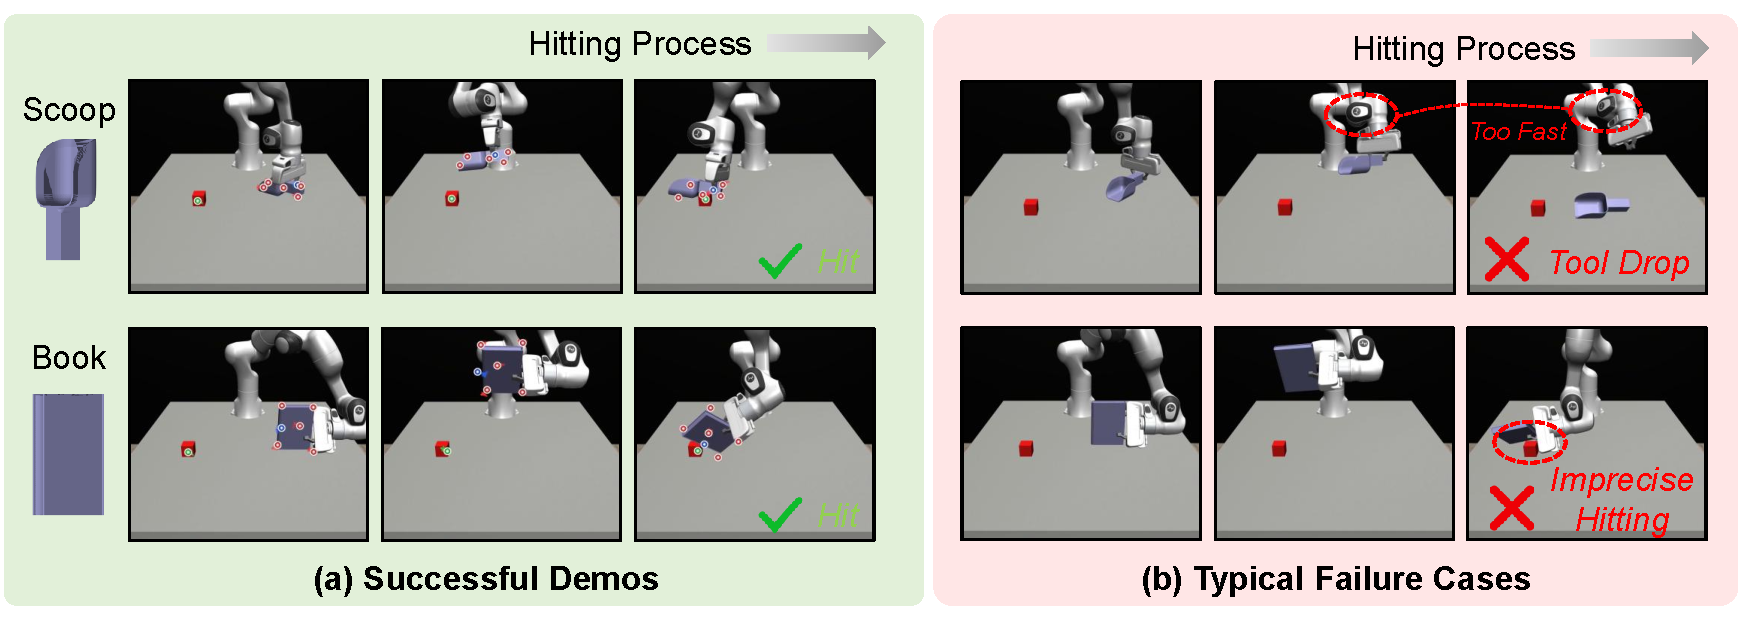
\includegraphics[width=0.95\linewidth]{figures/qualitative-results.pdf}
%     \caption{\textbf{Qualitative results of \algoname{}.} (a) Successful demos with predicted keypoint-based functional plans on unseen tools. (b) Two typical failure cases of \algoname{}.}

%     \label{fig:qualitative-analysis}
% \end{figure}

% \subsection{Qualitative Analysis}

% In this section, we conduct a comprehensive qualitative analysis on the behavior of \algoname{} on unseen tools. 
% As shown in Fig.~\ref{fig:qualitative-analysis}, we first visualize the predicted 2D keypoint-based functional plans of \algoname{} on different unseen tools. 
% We then summarize two representative failure cases from \algoname{}, which provide useful insights for further improvement.

% \subsubsection{Visualization of Functional Plans of \algoname{}.}

% Fig.~\ref{fig:qualitative-analysis}(a) visualizes the functional plans predicted by \algoname{} on unseen tools. 
% Although these tools are not observed during training, \algoname{} can still predict structured keypoint trajectories that reflect the underlying functional intent, such as aligning the hitting point with the target point before contact. 
% Conditioned on these predicted functional plans, the execution policy can ground them into robot actions and successfully complete the hitting task with the designated hitting point. 
% These results show that the learned keypoint-based plans capture transferable functional motion patterns beyond tool-specific appearances.

% \subsubsection{Typical Failure Cases.}

% As shown in Fig.~\ref{fig:qualitative-analysis}(b), we further identify two representative failure modes of our \algoname{}.

% \paragraph{Imprecise hitting.}
% The first failure mode is imprecise hitting. 
% Although \algoname{} can predict a roughly correct hitting trajectory, it may fail to strike the target precisely with the designated hitting point. 
% We conjecture that this limitation comes from the 2D keypoint representation, and exploring 3D-aware functional intermediate representations may further improve the performance.

% \paragraph{Tool dropping.}
% The second failure mode is tool dropping. 
% The low-level execution policy may ground the predicted functional plan into jerky actions, causing the tool to drop from the gripper and eventually fail the hitting task. 
% Introducing additional smoothness constraints during the finetuning of the low-level execution policy or applying post-processing to the predicted actions may help mitigate this problem.

% \subsection{Qualitative Analysis \lw{Failure Analysis}} 

% % We conduct a comprehensive qualitative analysis of \algoname{} on unseen tools and summarize representative failure cases in Fig.~\ref{fig}.

% %\paragraph{Functional Plan Visualization.}
% \textbf{Functional Plan Visualization.}~~
% As shown in Fig.~\ref{fig:qualitative-analysis}~(a), \algoname{} predicts structured keypoint-based functional plans for unseen tools such as the book and scoop. These plans capture transferable functional motion patterns, such as aligning the hitting region with the target before contact. Conditioned on the predicted plans, the execution policy grounds them into robot actions and successfully completes the hitting task with the designated hitting point.

% %\paragraph{Typical Failure Cases.}
% \textbf{Typical Failure Cases.}~~
% Fig.~\ref{fig:qualitative-analysis}~(b) reveals two representative failure modes of \algoname{}. The first is \textit{imprecise hitting}, where \algoname{} predicts a roughly correct hitting trajectory but fails to strike the target precisely with the designated hitting point. This suggests that 2D keypoints may be insufficient for fine-grained spatial alignment, and 3D-aware functional representations may further improve performance. The second is \textit{tool dropping}, where the execution policy grounds the predicted plan into jerky actions and causes the tool to slip from the gripper. This indicates that smoother action grounding or action post-processing may help improve low-level execution robustness.